\documentclass[a4paper,11pt,UTF8]{article}
\usepackage{ctex}
\usepackage{amsmath,amsthm,amssymb,amsfonts}
\usepackage{amsmath}
\usepackage[a4paper]{geometry}
\usepackage{graphicx}
\usepackage{microtype}
\usepackage{siunitx}
\usepackage{booktabs}
\usepackage[colorlinks=false, pdfborder={0 0 0}]{hyperref}
\usepackage{cleveref}
\usepackage{esint} 
\usepackage{graphicx}
\usepackage{ragged2e}
\usepackage{pifont}
\usepackage{extarrows}
\usepackage{mathptmx}
\usepackage{float}
\usepackage{caption}
\usepackage{bm}
\captionsetup[figure]{name={Figure}}
%opening
\title{科学计算引论作业(四)}
\author{谢悦晋 \quad U202210333}
\date{Oct 15th, 2023 }
\begin{document}
\maketitle
\textbf{3.10} (实验题) 给定线性方程组
$$
	\begin{pmatrix}
		1&2&3&4&5\\
		-2&3&4&5&6\\
		-3&-4&5&6&7\\
		-4&-5&-6&7&8\\
		-5&-6&-7&-8&9
	\end{pmatrix}
	\begin{pmatrix}x_1\\x_2\\x_3\\x_4\\x_5\end{pmatrix}
	=\begin{pmatrix}55\\66\\63\\36\\-25\end{pmatrix}.
$$

试以 $\|X^{(k+1)}-X^{(k)}\|_\infty<10^{-5}$ 作为终止准则,分别利用 Jacobi 迭代法、Gauss-Seidel 迭代法及具有最佳松弛因子的 JOR 迭代方法和 SOR 迭代法求解该方程组,并比较这些方法的计算时间.

解:Jacobi 迭代法、Gauss-Seidel 迭代法是无法收敛的,而JOR 迭代方法和 SOR 迭代法可以收敛,结果如下:
\begin{figure}[H]
	\centering
	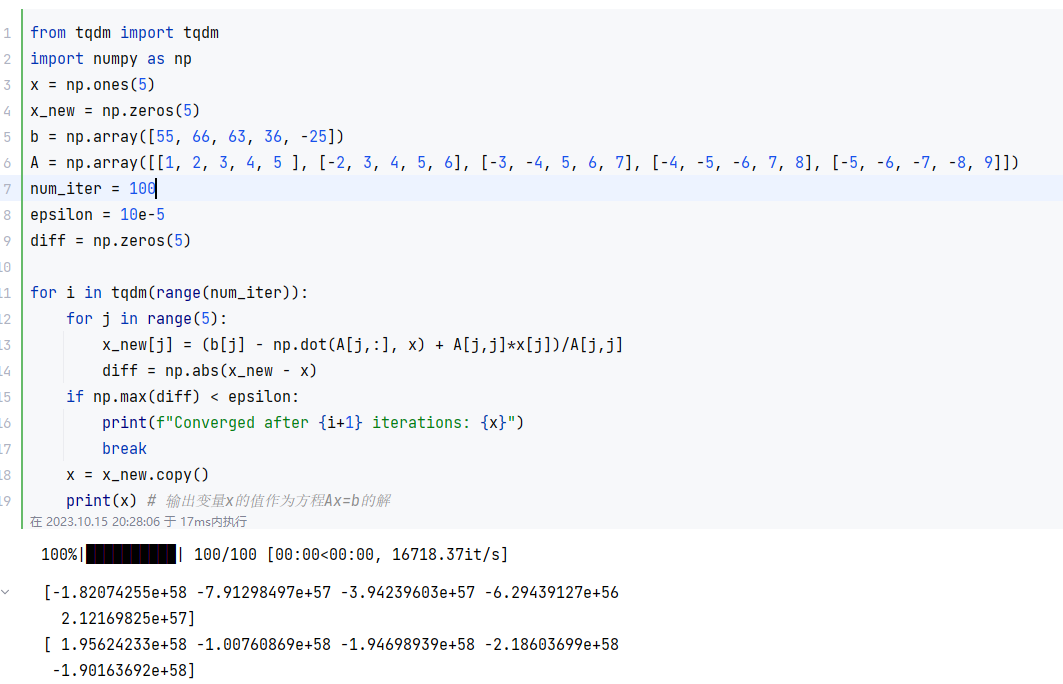
\includegraphics[scale=0.3]{3.10_1}
\end{figure}
\begin{figure}[H]
	\centering
	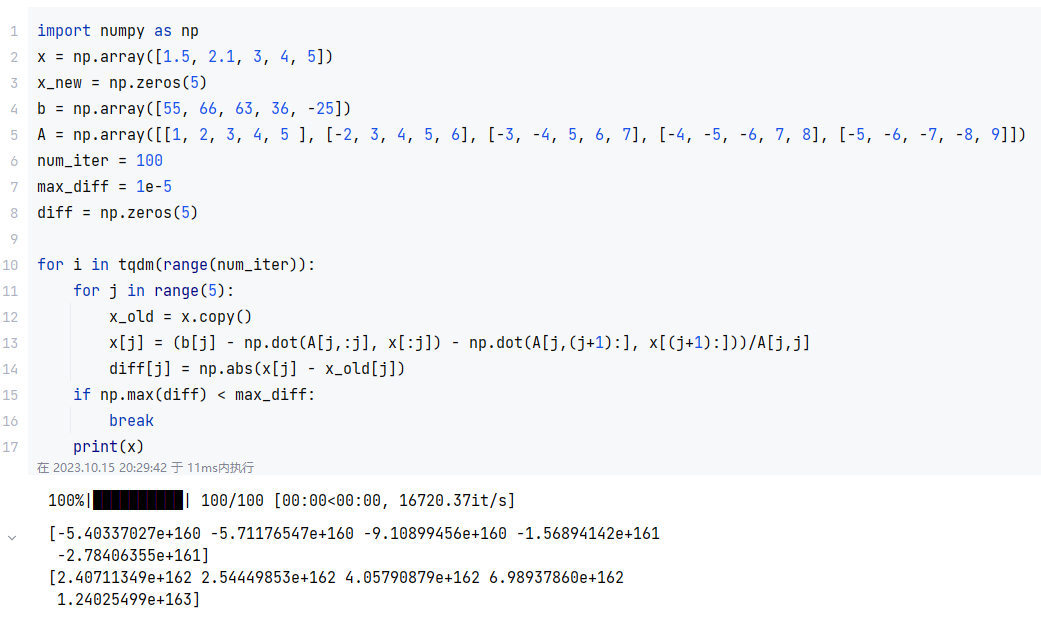
\includegraphics[scale=0.3]{3.10_2}
\end{figure}
\begin{figure}[H]
	\centering
	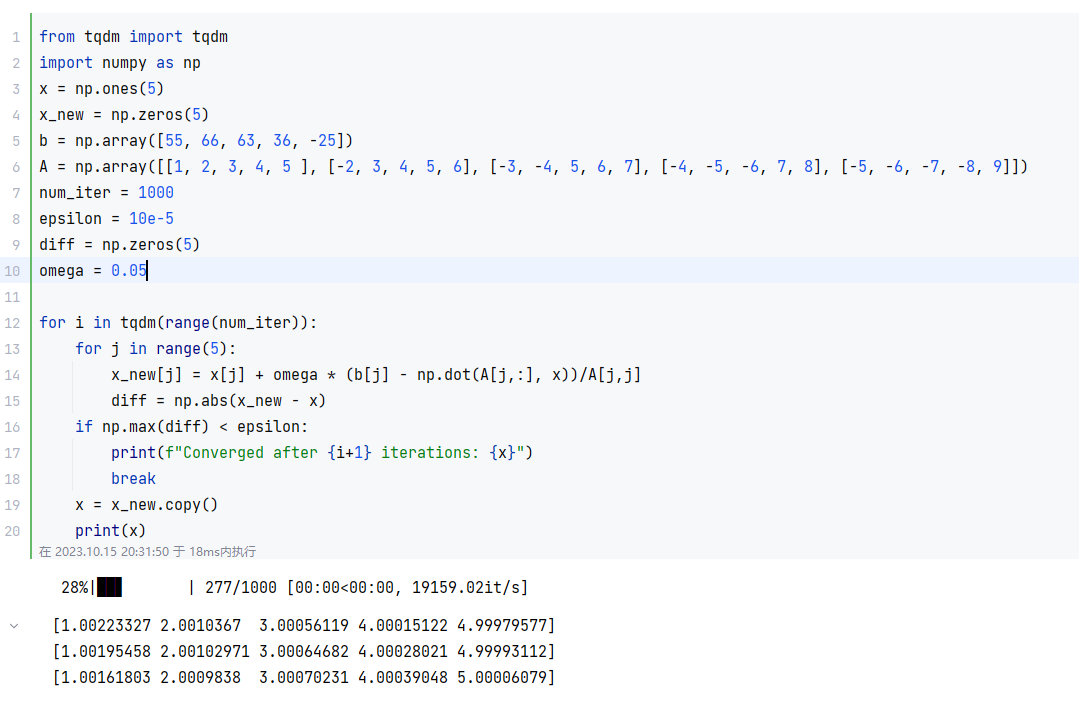
\includegraphics[scale=0.3]{3.10_3}
\end{figure}
\begin{figure}[H]
	\centering
	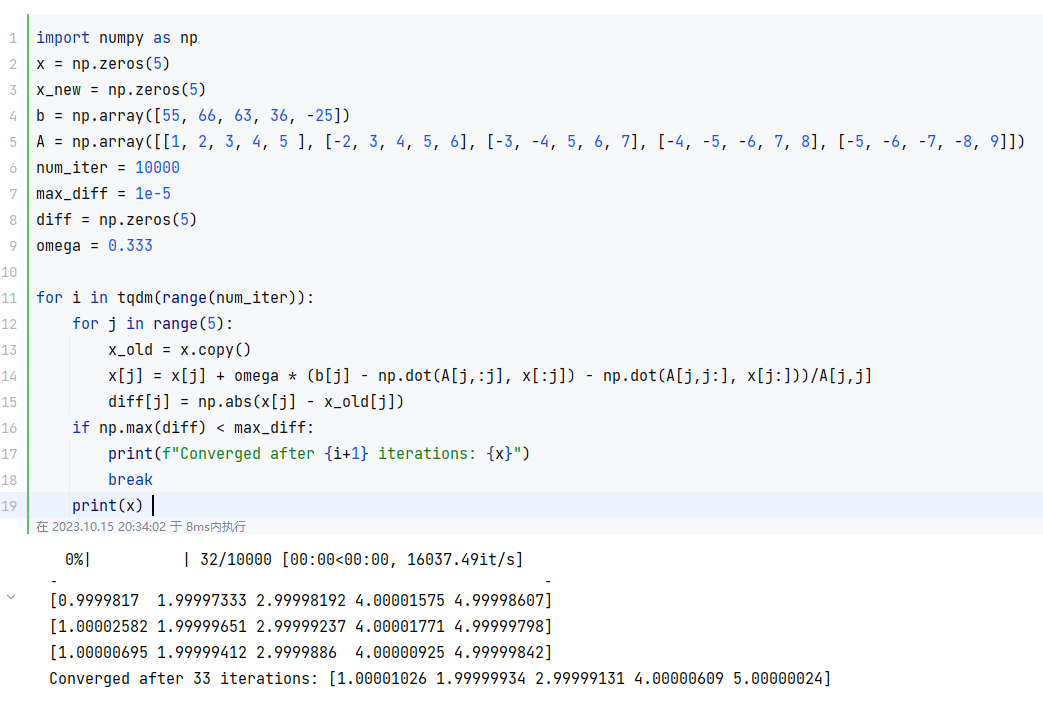
\includegraphics[scale=0.3]{3.10_4}
\end{figure}
\textbf{4.1} 给定函数 $f(x)=x\exp(x)(1+\exp(x))$ 及插值节点 $x_0=1.00,$ $x_{1}=1.02,x_{2}=1.04,x_{3}=1.06$,试构造 3 次 Lagrange 插值多项式计算$f(1.03)$ 的逼近值,并导出其误差估计.

解:

Lagrange插值多项式:
$$
	L_3(x)=\sum_{i=0}^3f(x_i)l_i(x),\quad l_i(x)=\prod_{j=0,j\neq i}^{3}\frac{(x-x_j)}{x_i-x_j}
$$

结果如下:
\begin{figure}[H]
	\centering
	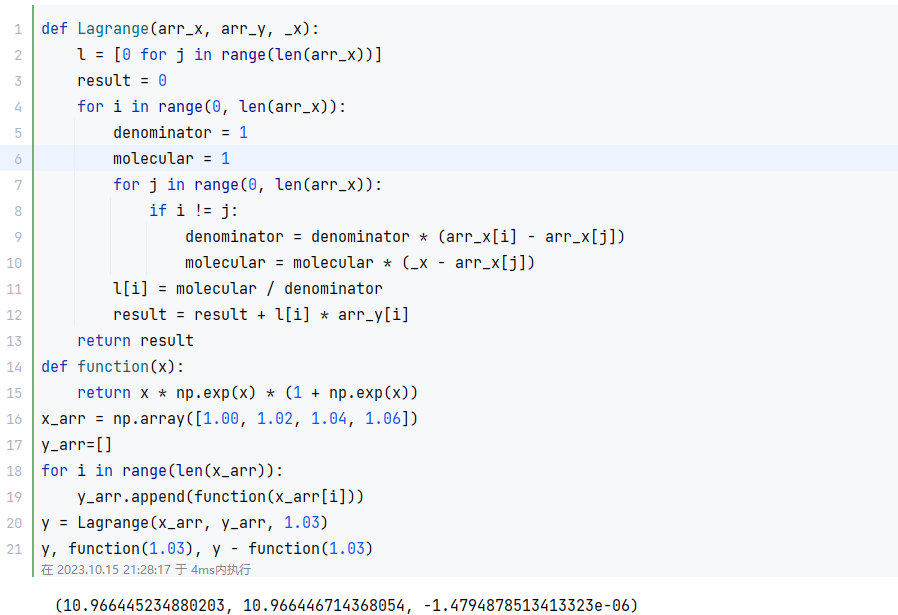
\includegraphics[scale=0.37]{4.1}
\end{figure}


\end{document}